\documentclass[a4paper,12pt,obeyspaces,spaces,hyphens]{article}

\def \trainingtype{online}
\def \agendalanguage{english}

\input{agenda/yocto.inc}

\usepackage{agenda}

\begin{document}

\feshowtitle

\feshowinfo

\feagendatwocolumn
{Hardware, first option}
{
  BeagleBone Black board
  \begin{itemize}
  \item An ARM AM335x processor from Texas Instruments (Cortex-A8
    based), 3D acceleration, etc.
  \item 512 MB of RAM
  \item 2 GB of on-board eMMC storage
        \newline(4 GB in Rev C)
  \item USB host and device
  \item HDMI output
  \item 2 x 46 pins headers, to access UARTs, SPI buses, I2C buses
    and more.
  \end{itemize}

}{}
{
  \begin{center}
    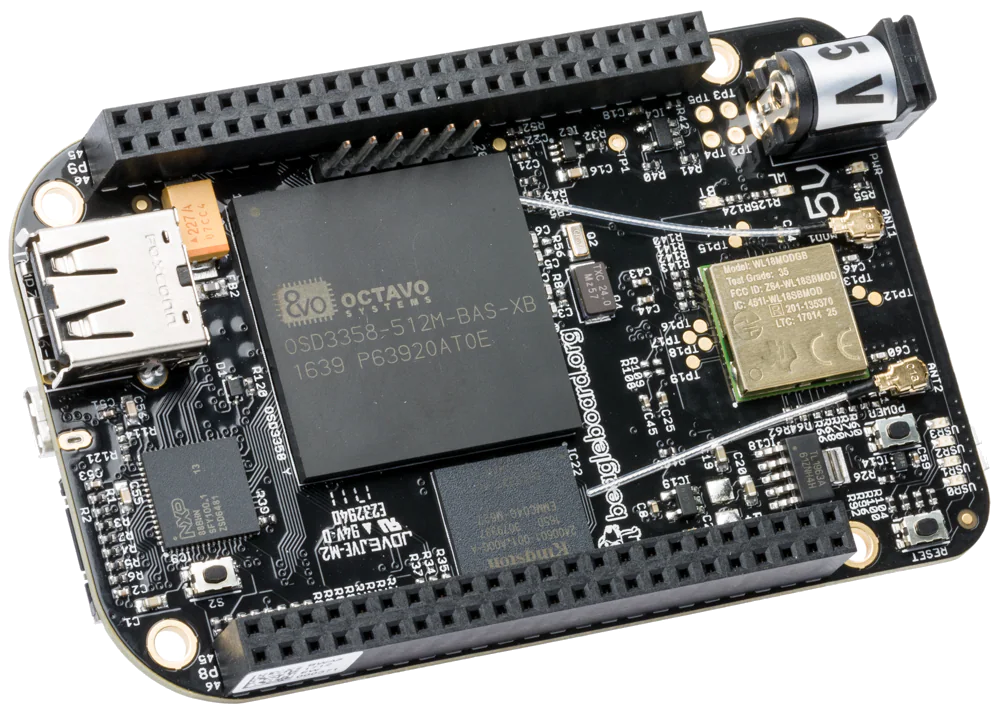
\includegraphics[width=5cm]{../slides/beagleboneblack-board/beagleboneblack.png}
  \end{center}
}

\feagendatwocolumn
{Hardware, second option}
{
  One of these Discovery Kits from STMicroelectronics: {\bf
  STM32MP157A-DK1}, {\bf STM32MP157D-DK1}, {\bf STM32MP157C-DK2} or
  {\bf STM32MP157F-DK2}
  \begin{itemize}
  \item STM32MP157 (dual Cortex-A7) CPU from STMicroelectronics
  \item USB powered
  \item 512 MB DDR3L RAM
  \item Gigabit Ethernet port
  \item 4 USB 2.0 host ports
  \item 1 USB-C OTG port
  \item 1 Micro SD slot
  \item On-board ST-LINK/V2-1 debugger
  \item Arduino Uno v3-compatible headers
  \item Audio codec
  \item Misc: buttons, LEDs
  \item LCD touchscreen (DK2 kits only)
  \end{itemize}
}{}
{
  \begin{center}
    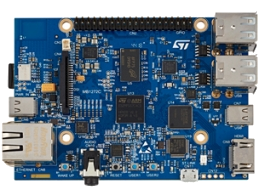
\includegraphics[width=5cm]{../slides/discovery-board-dk1/discovery-board-dk1.png}
  \end{center}
}

\section{Half day 1}

\feagendaonecolumn
{Lecture - Introduction to embedded Linux build systems}
{
  \begin{itemize}
  \item Overview of an embedded Linux system architecture
  \item Methods to build a root filesystem image
  \item Usefulness of build systems
  \end{itemize}
}

\feagendaonecolumn
{Lecture - Yocto Project and Poky reference system overview}
{
  \begin{itemize}
  \item Introduction to the Yocto / OpenEmbedded build system and its lexicon
  \item Overview of the Poky reference system
  \end{itemize}
}

\feagendatwocolumn
{Lecture - Using Yocto Project - basics}
{
  \begin{itemize}
  \item Setting up the build directory and environment
  \item Configuring the build system
  \item Building a root filesystem image using the Yocto Project
  \end{itemize}
}
{Demo 1 - First Yocto Project build}
{
  \begin{itemize}
  \item Downloading the Poky reference build system
  \item Configuring the build system
  \item Building a system image
 \end{itemize}
}

\feagendatwocolumn
{Lecture - Using Yocto Project - basics}
{
  \begin{itemize}
  \item Organization of the build output
  \end{itemize}
}
{Demo 1 - Flashing and booting}
{
  \begin{itemize}
  \item Flashing and booting the image on the board
  \end{itemize}
}

\newpage
\section{Half day 2}

\feagendatwocolumn
{Lecture - Using Yocto Project - advanced usage}
{
  \begin{itemize}
  \item Variable assignment, operators and overrides
  \item Package variants and package selection
  \item bitbake command line options
  \end{itemize}
}
{Demo 2 - Using NFS and configuring the build}
{
  \begin{itemize}
  \item Configuring the board to boot over NFS
  \item Add a package to the root filesystem
  \item Learn how to use the \code{PREFERRED_PROVIDER} mechanism
  \item Get familiar with the bitbake command line options
  \end{itemize}
}
\\

\feagendatwocolumn
{Lecture - Writing recipes - basics}
{
  \begin{itemize}
  \item Recipes: overview
  \item Recipe file organization
  \item Applying patches
  \item Recipe examples
  \end{itemize}
}
{Demo 3 - Adding an application to the build}
{
  \begin{itemize}
  \item Writing a recipe for {\em nInvaders}
  \item Troubleshooting the recipe
  \item Troubleshooting cross-compilation issues
  \item Adding {\em ninvaders} to the final image
  \end{itemize}
}

\feagendaonecolumn
{Lecture - Writing recipes - advanced features}
{
  \begin{itemize}
  \item Extending and overriding recipes
  \item Virtual packages
  \item Learn about classes
  \item BitBake file inclusions
  \item Debugging recipes
  \item Configuring bitbake network usage
  \end{itemize}
}

\section{Half day 3}

\feagendatwocolumn
{Lecture - Layers}
{
  \begin{itemize}
  \item What layers are
  \item Where to find layers
  \item Creating a layer
  \end{itemize}
}
{Demo 4 - Writing a layer}
{
  \begin{itemize}
  \item Learn how to write a layer
  \item Add the layer to the build
  \item Move {\em ninvaders} to the new layer
  \end{itemize}
}

\feagendaonecolumn
{Demo 5 - Extend a recipe}
{
  \begin{itemize}
  \item Extend the kernel recipe to add patches
  \item Configure the kernel to compile the nunchuk driver
  \item Edit the ninvaders recipe to add patches
  \item Play {\em nInvaders}
  \end{itemize}
}

\feagendatwocolumn
{Lecture - Writing a BSP}
{
  \begin{itemize}
  \item Introduction to BSP layers
  \item Adding a new machine
  \item Bootloader configuration
  \item Linux: the kernel bbclass and the linux-yocto recipe
  \end{itemize}
}
{Demo 6 - Create a custom machine configuration}
{
  \begin{itemize}
  \item Create a new machine configuration
  \item Build an image for the new machine
  \end{itemize}
}

\feagendaonecolumn
{Lecture - Distro layers}
{
  \begin{itemize}
  \item Distro configuration
  \item Distro layers
  \item Automating layer management
  \end{itemize}
}

\feagendatwocolumn
{Lecture - Images}
{
  \begin{itemize}
  \item Writing an image recipe
  \item Image types
  \item Writing and using package groups recipes
  \end{itemize}
}
{Demo 7 - Create a custom image}
{
  \begin{itemize}
  \item Add a basic image recipe
  \item Select the images capabilities and packages
  \item Add a custom package group
  \item Add an image variant for debugging
  \end{itemize}
}

\section{Half day 4}

\feagendatwocolumn
{Lecture - Writing recipes - going further}
{
  \begin{itemize}
  \item The per-recipe sysroot
  \item Using Python code in metadata
  \item Variable flags
  \item Packages features and PACKAGECONFIG
  \item Conditional features
  \item Package splitting
  \item Dependencies in detail
  \end{itemize}
}
{Lecture - Licensing}
{
  \begin{itemize}
  \item Managing open source licenses
  \end{itemize}
}

\feagendatwocolumn
{Lecture - Application development workflows}
{
  \begin{itemize}
  \item The Yocto Project SDK
  \item Devtool
  \item Quilt
  \end{itemize}
}
{Demo 8 - Develop your application in the Poky SDK}
{
  \begin{itemize}
  \item Building an SDK
  \item Using the Yocto Project SDK
  \end{itemize}
}

\feagendatwocolumn
{Lecture - Automating layer management}
{
  \begin{itemize}
  \item Automating layer management
  \end{itemize}
}
{Lecture - Runtime Package Management}
{
  \begin{itemize}
  \item Introduction to runtiome package management
  \item Build configuration
  \item Package server configuration
  \item Target configuration
  \end{itemize}
}

\feagendaonecolumn
{Questions and Answers}
{
  \begin{itemize}
  \item Questions and answers with the audience about the course topics
  \item Extra presentations if time is left, according what most
        participants are interested in.
  \end{itemize}
}

\section{Possible extra time}

{\em Extra time (up to 4 hours) may be proposed if the agenda didn't fit in 4 half days,
     according to the time spent answering questions from participants.}

\end{document}

